\section{Color Predictions}
\label{sec:color_predicts}

Using the text name of a card, I aimed to predict
which of the five colors (or null) that card would be.
I had to take into account a couple considerations in
constructing my network and dataset. First, a text name
is not something I can immediately feed into a neural net.
Second, I am working with a small dataset of approximately
18,000 unique cards. And finally, some cards have multiple
colors, which might mean they need to be treated specially.

\subsection{Fully Connected Architecture}
Confronting the first issue I mentioned above, I decided to use 
Word2Vec to translate the card names into vector form. Throughout
my project, I experimented with many different implementations of 
word to vector which I will document with each architecture. To start,
I used Word2Vec's pretrained model which learned from english Wikipedia
and has 1,000 dimensions\cite{deeplearning4j}. Using this model has issues:
primarily, not all the names in the Magic universe have an equivalent 
vector in the trained model. For these cards, I chose to ignore those words.
Then, any cards that have no vector form at all, I remove from my dataset.
While trimming an already small dataset is not the best practice, it was a
necessary step to take at the time. I also lost 94 words due to lack of UTF8
compatibility -- cards with characters an umlaut for example would cause problems
in the Word2Vec model. This model had an space problem of being
8GB large, leading to long loading and preprocessing times.

The first architecture I worked with was a single layer of
300 nodes, and a 20\% dropout layer. I used a sigmoid activation
function, learning rate of 0.001, and the Adam optimizer. Over time
I changed the number of layers to 3, using 150, 100, and 50 nodes in
each layer. I replaced the sigmoid with tanh then relu and increased
the dropout layer to 60\% (with dropout between each layer). This model
is shown in the appendix for clarity.

\subsection{The Dataset}
I found my initial dataset from Kaggle Datasets. It contained
a list of 8,000 cards printed from 1995-2007. At the time, I
didn't realize I was only working with about 50\% of all cards
printed, but when I did realize my mistake, the data I received 
provided interesting enough insights into the evolution of the game 
that I figure they are worth noting below.
Using the above architecture and this dataset, I trained on 7,000 card name 
vectors and tested with 1338, outputting a color vector. My network 
plateaued at 60\% accuracy (random baseline of 18\%).

After getting this initial result, I spent more time looking for
a better, more complete catalog. In the end, I used MTGJson\cite{mtgjson}.
With the new dataset I have about 18,000 cards from 1995-2017. 
I separated this into 15,000 training and 3,000 testing (randomly shuffled).
My model achieved 54\% accuracy.

It was interesting to me that the full set of cards actually had lower accuracy
than the half set of cards. My two proposed explanations of this are that
either the network was lucker in the first training case (the training and test
data had an easier split) or that over the course of the last 10 years, the 
creators of Magic the Gathering have taken more liberties with what the color
of a card represents.

\subsection{New Text Models}
The next variable I manipulated was the word to vector model I was using.
Searching around, I found a model trained on Google News. Each vector is 300
dimensions. Approximately 1,800 cards were ignored due to unknown names with 
this model. Using the same 150--100--50 architecture as above, this model
received 50\% accuracy. Even though it has 4\% loss in accuracy, the 
advantage of this model is only being 2GB of space, compared to the 8GB
for the 1,000 dimension Wikipedia model. I looked into Stanford's 
training model as well: Glove\cite{pennington2014glove}.
Using this 300 dimension model, I was able to achieve 54\% accuracy. 
For practical purposes, Glove is the model I used from here on out due 
to its performance and 2GB memory footprint.

\begin{figure}[h!]
    \centering
    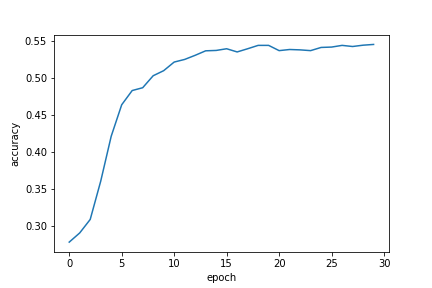
\includegraphics[width=0.9\linewidth]{figures/glove_color.png}
    \caption{Glove, 150--100--50}
    \label{fig:glove_color}
\end{figure}
